\documentclass[ignorenonframetext,]{beamer}
\setbeamertemplate{caption}[numbered]
\setbeamertemplate{caption label separator}{: }
\setbeamercolor{caption name}{fg=normal text.fg}
\beamertemplatenavigationsymbolsempty
\usepackage{lmodern}
\usepackage{amssymb,amsmath}
\usepackage{ifxetex,ifluatex}
\usepackage{fixltx2e} % provides \textsubscript
\ifnum 0\ifxetex 1\fi\ifluatex 1\fi=0 % if pdftex
\usepackage[T1]{fontenc}
\usepackage[utf8]{inputenc}
\else % if luatex or xelatex
\ifxetex
\usepackage{mathspec}
\else
\usepackage{fontspec}
\fi
\defaultfontfeatures{Ligatures=TeX,Scale=MatchLowercase}
\fi
\usetheme{gcat}
% use upquote if available, for straight quotes in verbatim environments
\IfFileExists{upquote.sty}{\usepackage{upquote}}{}
% use microtype if available
\IfFileExists{microtype.sty}{%
\usepackage{microtype}
\UseMicrotypeSet[protrusion]{basicmath} % disable protrusion for tt fonts
}{}
\newif\ifbibliography
\usepackage{longtable,booktabs}
\usepackage{caption}
% These lines are needed to make table captions work with longtable:
\makeatletter
\def\fnum@table{\tablename~\thetable}
\makeatother
\usepackage{graphicx,grffile}
\makeatletter
\def\maxwidth{\ifdim\Gin@nat@width>\linewidth\linewidth\else\Gin@nat@width\fi}
\def\maxheight{\ifdim\Gin@nat@height>\textheight0.8\textheight\else\Gin@nat@height\fi}
\makeatother
% Scale images if necessary, so that they will not overflow the page
% margins by default, and it is still possible to overwrite the defaults
% using explicit options in \includegraphics[width, height, ...]{}
\setkeys{Gin}{width=\maxwidth,height=\maxheight,keepaspectratio}

% Prevent slide breaks in the middle of a paragraph:
\widowpenalties 1 10000
\raggedbottom

\AtBeginPart{
\let\insertpartnumber\relax
\let\partname\relax
\frame{\partpage}
}
\AtBeginSection{
\ifbibliography
\else
\let\insertsectionnumber\relax
\let\sectionname\relax
\frame{\sectionpage}
\fi
}
\AtBeginSubsection{
\let\insertsubsectionnumber\relax
\let\subsectionname\relax
\frame{\subsectionpage}
}

\setlength{\parindent}{0pt}
\setlength{\parskip}{6pt plus 2pt minus 1pt}
\setlength{\emergencystretch}{3em}  % prevent overfull lines
\providecommand{\tightlist}{%
\setlength{\itemsep}{0pt}\setlength{\parskip}{0pt}}
\setcounter{secnumdepth}{0}

\title{Significant pattern mining on GWAS data}
\author{Xavier Duran\\
GCAT Genomes for Life\\
Institut de Recerca Germans Trias i Pujol (IGTP)}
\date{Bioinfo Talks\\
February 15\textsuperscript{th} 2017}

\begin{document}
\frame{\titlepage}

\begin{frame}{Missing heritability problem on GWAS}

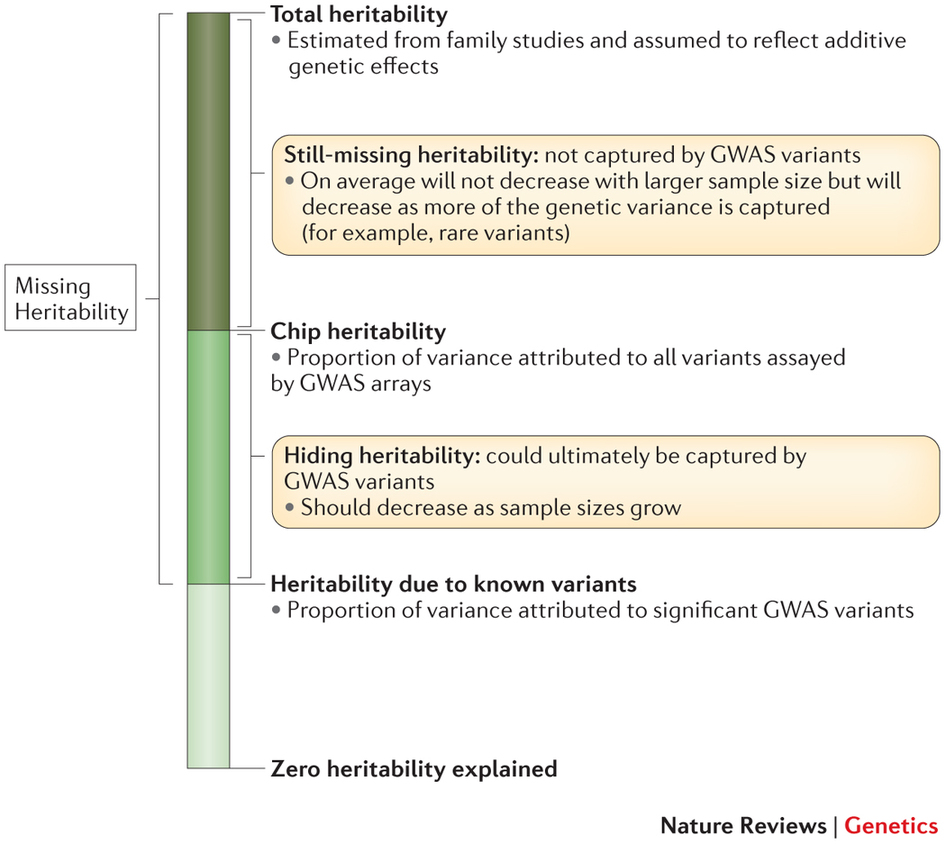
\includegraphics{images/nrg3786-f4.jpg}

\end{frame}

\begin{frame}{Limitless arity multi-testing procedure (LAMP)}

Significant pattern mining techniques can help to find high-order
interactions on GWAS data (and other biological data)

\pause

\begin{block}{Outline}

The complexity of combinatorial variant discovery

\pause

How does LAMP approaches a solution

\pause

Results on a lung cancer dataset

\end{block}

\end{frame}

\begin{frame}{Finding combinations of features}

\begin{block}{Computational problem}

Exploring all combinations is computationally prohibitive

\pause

\(M^2\) second order possible interactions

\pause

\(2^M\) limitless order interactions

\pause

\end{block}

\begin{block}{Statistical problem}

Discovered combinations are statistically unlikely due to multiple
testing correction

\pause

For \(M\) binary variables, Bonferroni correction sets significance
below \(\frac{\alpha}{2^M}\)

\end{block}

\end{frame}

\begin{frame}{Finding combinations of features}

\begin{block}{Machine learning approaches}

Random Forests, Support Vector Machines, Multifactor Dimensionality
Reduction

\pause

Variable rankings

\pause

Too many false positives

\pause

Very costly to further explore hypothesis

\end{block}

\end{frame}

\begin{frame}{Limitless arity multi-testing procedure (LAMP)}

11\(S=\{SNP_1, SNP_2,...,SNP_n\}\), n is the arity of the combination

\pause

\begin{block}{Fisher's exact test}

Not all combinations are frequent enough to become significant in any
case/control setting

\pause

\begin{longtable}[]{@{}lrrr@{}}
\toprule
& Case & Control & Total\tabularnewline
\midrule
\endhead
Has \(S\) & & & 13\tabularnewline
Hasn't \(S\) & & & 357\tabularnewline
total & 184 & 186 & 370\tabularnewline
\bottomrule
\end{longtable}

\end{block}

\end{frame}

\begin{frame}{Limitless arity multi-testing procedure (LAMP)}

\(S=\{SNP_1, SNP_2,...,SNP_n\}\), n is the arity of the combination

\begin{block}{Fisher's exact test}

Not all combinations are frequent enough to become significant in any
case/control setting

\begin{longtable}[]{@{}lrrr@{}}
\toprule
& Case & Control & Total\tabularnewline
\midrule
\endhead
Has \(S\) & 13 & 0 & 13\tabularnewline
Hasn't \(S\) & 171 & 186 & 357\tabularnewline
total & 184 & 186 & 370\tabularnewline
\bottomrule
\end{longtable}

\pause

raw p-value = \(9.1*10^{-5}\)

\pause

FWER threshold \(\delta=\alpha/1000\) = 0.05/1000 = \(5*10^{-5}\)

\end{block}

\end{frame}

\begin{frame}{Limitless arity multi-testing procedure (LAMP)}

Multiple testing procedure for listing ALL statistically significant
high order interactions

\pause

Upper bound of Family Wise Error Ratio (FWER)

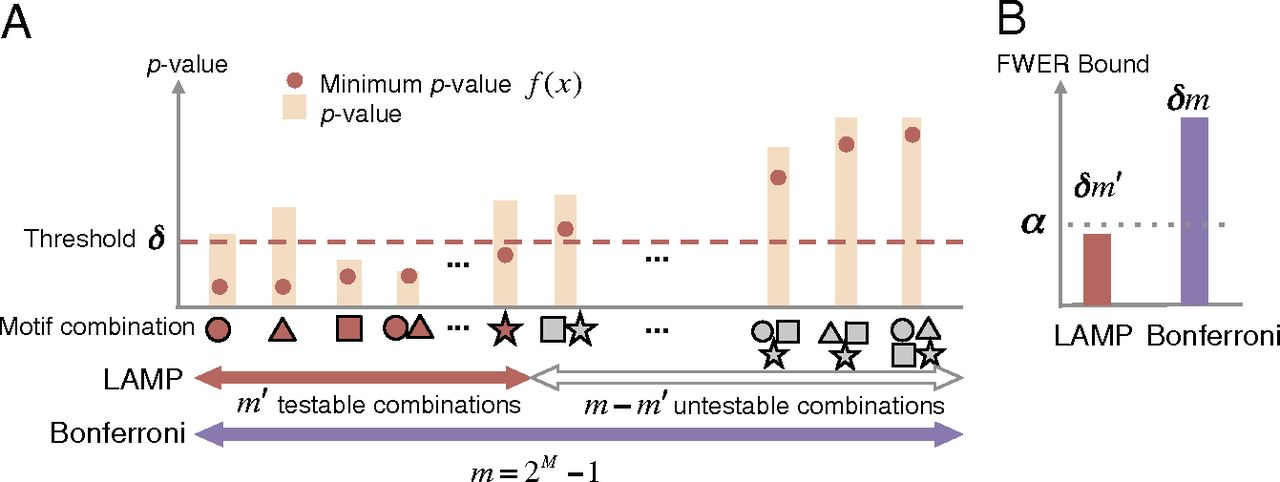
\includegraphics{images/F2.large.jpg}

{[}Terada et al. 2013{]}

\end{frame}

\begin{frame}{LAMPLINK}

LAMPLINK is implemented as additional features to PLINK

\pause

Model dominant/recessive for the risk class for the minor allele

\pause

\begin{block}{Algorithm}

Find all significant combinations

\pause

Remove combinations with SNPs in linkage disequilibrium
(\(r^2 < threshold\))

\end{block}

\end{frame}

\begin{frame}{LAMPLINK}

\begin{block}{Progression of non-small cell lung cancer (NSCLC) GWAS
data}

\begin{longtable}[]{@{}ll@{}}
\toprule
GWAS threshold & p-value \textless{} \(10^{-4}\)\tabularnewline
SNPs & 695\tabularnewline
Individuals & 178\tabularnewline
Statistical test & Fisher's exact test\tabularnewline
Adjusted significance level & \(5.8*10^{-9}\)\tabularnewline
Correction factor & 8619336\tabularnewline
Significant combinations & 5019\tabularnewline
\(r^2\) for LD & 0.2\tabularnewline
Significant combinations after LD pruning & 145\tabularnewline
Significant SNPs & 25\tabularnewline
Maximum arity & 7\tabularnewline
\bottomrule
\end{longtable}

\end{block}

\end{frame}

\begin{frame}{LAMPLINK}

\begin{block}{Progression of non-small cell lung cancer (NSCLC) GWAS
data}

\begin{table}[ht]
\centering
\scalebox{0.4}{
\begin{tabular}{rlr}
  \hline
Adjusted\_P & COMB & arity \\ 
  \hline
0.00001538 & rs438228:161484124:A:C,rs35684:10326686:A:G,rs1565656:188922545:A:G,rs4545589,rs139996291:17192744:G:A & 5 \\ 
  0.00002144 & rs2271545:16095316:C:T,rs438228:161484124:A:C,rs35684:10326686:A:G,rs1565656:188922545:A:G & 4 \\ 
  0.00004028 & rs438228:161484124:A:C,rs35684:10326686:A:G,rs1565656:188922545:A:G,rs4545589,rs9788969,rs139996291:17192744:G:A & 6 \\ 
  0.00008586 & rs2271545:16095316:C:T,rs35684:10326686:A:G,rs1565656:188922545:A:G,rs139996291:17192744:G:A & 4 \\ 
  0.00009664 & rs35684:10326686:A:G,rs1565656:188922545:A:G,rs4545589,rs9788969,rs139996291:17192744:G:A & 5 \\ 
  0.00011584 & rs35684:10326686:A:G,rs1565656:188922545:A:G,rs4545589,rs139996291:17192744:G:A & 4 \\ 
  0.00013264 & rs2271545:16095316:C:T,rs438228:161484124:A:C,rs35684:10326686:A:G,rs1565656:188922545:A:G,rs139996291:17192744:G:A & 5 \\ 
  0.00025099 & rs2937667:117246037:C:A,rs10985542:124887090:G:A,12:48798429:T:C,rs139996291:17192744:G:A & 4 \\ 
  0.00050371 & rs35684:10326686:A:G,rs2937667:117246037:C:A,rs1565656:188922545:A:G,rs139996291:17192744:G:A & 4 \\ 
  0.00058472 & rs438228:161484124:A:C,rs35684:10326686:A:G,rs1565656:188922545:A:G,rs4545589,rs9788969 & 5 \\ 
  0.00058472 & rs438228:161484124:A:C,rs35684:10326686:A:G,rs6822954:35695840:A:G,rs1565656:188922545:A:G,rs4545589 & 5 \\ 
  0.00067780 & rs1565656:188922545:A:G,rs7111257:9930813:A:G,rs4545589,rs139996291:17192744:G:A & 4 \\ 
  0.00078732 & rs2271545:16095316:C:T,rs438228:161484124:A:C,rs35684:10326686:A:G,rs1565656:188922545:A:G,rs9788969 & 5 \\ 
  0.00078732 & rs35684:10326686:A:G,rs2937667:117246037:C:A,rs1565656:188922545:A:G,rs4545589,rs139996291:17192744:G:A & 5 \\ 
  0.00078732 & rs35684:10326686:A:G,rs2937667:117246037:C:A,rs1565656:188922545:A:G,rs71317450:27405120:A:T,rs139996291:17192744:G:A & 5 \\ 
  0.00078732 & rs35684:10326686:A:G,rs6822954:35695840:A:G,rs1565656:188922545:A:G,rs4545589 & 4 \\ 
  0.00079983 & rs2271545:16095316:C:T,rs35684:10326686:A:G,rs1565656:188922545:A:G,rs9788969,rs139996291:17192744:G:A & 5 \\ 
  0.00079983 & rs35684:10326686:A:G,rs6822954:35695840:A:G,rs11740157:10041128:A:G,12:51088287:AATACATAC:A & 4 \\ 
  0.00117950 & rs438228:161484124:A:C,rs1565656:188922545:A:G,rs4545589,rs139996291:17192744:G:A & 4 \\ 
  0.00151520 & rs2937667:117246037:C:A,rs10985542:124887090:G:A,12:48798429:T:C,rs9788969,rs139996291:17192744:G:A & 5 \\ 
   \hline
\end{tabular}
}
\caption{Top 20 statistically significant variant combinations} 
\end{table}

\end{block}

\end{frame}

\begin{frame}{LAMPLINK}

\begin{block}{Progression of non-small cell lung cancer (NSCLC) GWAS
data}

\begin{table}[ht]
\centering
\scalebox{0.4}{
\begin{tabular}{rrlllrllrrrr}
  \hline
CHR & BP & SNP & A1 & A2 & MAF & AFF & UNAFF & P\_FISHER & P\_GWAS & OR & COMB \\ 
  \hline
22 & 17192744 & rs139996291:17192744:G:A & A & G & 0.3649890 & 34/7 & 74/62 & 0.00094253 & 0.0000210682 & 4.06950 & 106 \\ 
  4 & 188922545 & rs1565656:188922545:A:G & G & A & 0.3507380 & 33/8 & 74/62 & 0.00327766 & 0.0000805378 & 3.45608 & 92 \\ 
  3 & 10326686 & rs35684:10326686:A:G & G & A & 0.2538130 & 30/11 & 56/80 & 0.00035202 & 0.0000464813 & 3.89610 & 88 \\ 
  16 & 88812250 & rs9788969 & C & T & 0.3649430 & 34/7 & 72/64 & 0.00051405 & 0.0000467814 & 4.31746 & 56 \\ 
  1 & 161484124 & rs438228:161484124:A:C & C & A & 0.3755220 & 32/9 & 77/59 & 0.01679720 & 0.0000519295 & 2.72439 & 49 \\ 
  1 & 16095316 & rs2271545:16095316:C:T & C & T & 0.3055050 & 32/9 & 64/72 & 0.00058287 & 0.0000858186 & 4.00000 & 41 \\ 
  11 & 87018161 & rs4545589 & G & A & 0.2931030 & 28/13 & 57/79 & 0.00409010 & 0.0000384487 & 2.98516 & 41 \\ 
  12 & 51088287 & 12:51088287:AATACATAC:A & AATACATAC & A & 0.3702890 & 33/8 & 79/57 & 0.00967982 & 0.0000061165 & 2.97627 & 36 \\ 
  3 & 117246037 & rs2937667:117246037:C:A & C & A & 0.3430310 & 32/9 & 77/59 & 0.01679720 & 0.0000190999 & 2.72439 & 32 \\ 
  5 & 10041128 & rs11740157:10041128:A:G & G & A & 0.2049100 & 27/14 & 42/94 & 0.00009612 & 0.0000475494 & 4.31633 & 31 \\ 
  4 & 35695840 & rs6822954:35695840:A:G & G & A & 0.3519970 & 33/8 & 68/68 & 0.00055543 & 0.0000719665 & 4.12500 & 15 \\ 
  9 & 124887090 & rs10985542:124887090:G:A & G & A & 0.2295800 & 26/15 & 49/87 & 0.00224055 & 0.0000826039 & 3.07755 & 13 \\ 
  12 & 48798429 & 12:48798429:T:C & T & C & 0.1586230 & 21/20 & 33/103 & 0.00174931 & 0.0000692089 & 3.27727 & 12 \\ 
  21 & 27405120 & rs71317450:27405120:A:T & T & A & 0.0950701 & 30/11 & 82/54 & 0.14438900 & 0.0002445401 & 1.79601 & 9 \\ 
  21 & 27405120 & rs71317450:27405120:A:T & T & A & 0.3784690 & 30/11 & 82/54 & 0.14438900 & 0.0002445401 & 1.79601 & 9 \\ 
  12 & 48792747 & 12:48792747:A:G & A & G & 0.1637820 & 21/20 & 33/103 & 0.00174931 & 0.0000424999 & 3.27727 & 7 \\ 
  5 & 10054699 & rs11744968:10054699:T:C & C & T & 0.1770790 & 23/18 & 36/100 & 0.00064061 & 0.0000862621 & 3.54938 & 5 \\ 
  11 & 9930813 & rs7111257:9930813:A:G & A & G & 0.2614450 & 29/12 & 56/80 & 0.00120037 & 0.0000422449 & 3.45238 & 5 \\ 
  16 & 78692994 & rs59689196:78692994:A:C & C & A & 0.1489970 & 18/23 & 27/109 & 0.00366244 & 0.0000446349 & 3.15942 & 5 \\ 
  4 & 161256788 & rs28657552:161256788:G:A & A & G & 0.3567330 & 31/10 & 69/67 & 0.00661204 & 0.0000510835 & 3.01014 & 3 \\ 
  13 & 41026812 & rs41286971:41026812:G:A & A & G & 0.3478880 & 30/11 & 74/62 & 0.04572730 & 0.0000474201 & 2.28501 & 3 \\ 
  17 & 12974799 & rs8065393:12974799:T:C & C & T & 0.3277870 & 32/9 & 65/71 & 0.00063784 & 0.0000359785 & 3.88376 & 3 \\ 
  11 & 8176765 & rs61400460:8176765:TA:T & T & TA & 0.0963394 & 18/23 & 11/125 & 0.00000071 & 0.0000483534 & 8.89328 & 2 \\ 
  21 & 36714156 & rs2242720 & G & A & 0.2729890 & 30/11 & 59/77 & 0.00118010 & 0.0009028600 & 3.55932 & 2 \\ 
  11 & 86367530 & rs9943610:86367530:C:T & C & T & 0.2151560 & 24/17 & 47/89 & 0.01033820 & 0.0000887781 & 2.67334 & 1 \\ 
  13 & 108513537 & rs1464811:108513537:A:G & G & A & 0.2638090 & 25/16 & 50/86 & 0.00706479 & 0.0000901488 & 2.68750 & 1 \\ 
   \hline
\end{tabular}
}
\caption{Variants statistically significant in any combination} 
\end{table}

\end{block}

\end{frame}

\begin{frame}{LAMPLINK}

\begin{block}{Progression of non-small cell lung cancer (NSCLC) GWAS
data}

NSCLC literature (mostly asian studies)

ELAC2 and HS3ST3A1 on the 50kb window of rs8065393

No significant pathways enriched

\end{block}

\end{frame}

\begin{frame}{Summary}

SNP combined effects may explain a part of the missing heritability but
is a computationally and statistically challenging problem

Significant pattern mining can help finding statistically significant
combinations of SNPs

The methodology is valid for other types of biomedical data

\end{frame}

\end{document}
